%%%%%%%%%%%%%%%%%%%%
%%%%% PREAMBLE %%%%%
%%%%%%%%%%%%%%%%%%%%

% Use the beamer class and configure it
\documentclass[aspectratio=169]{beamer}
\setbeamertemplate{section in toc}[square]
\setbeamertemplate{subsection in toc}[square]
\setbeamercolor{subsection in toc}{fg=alerted text.fg}
\setbeamercolor{subsection in toc shaded}{fg=structure}

% Use the metropolis theme and configure it
\usetheme
    [
      titleformat = smallcaps,
      numbering = fraction,
      progressbar = foot,
      block = fill
    ]
    {metropolis}

\usepackage[font={scriptsize,it}, labelfont={scriptsize,it}, justification=centering]{caption}
\usepackage{booktabs}
\usepackage{ragged2e}

% Presentation main information
\title{Static Analysis Tool Exposition (SATE)\\Test Case Development}
\date{December 2\textsuperscript{nd}, 2017}
\author{\textbf{Damien Cupif}}
\institute{\textbf{\textit{Oral Defense for TELECOM Nancy Master's Degree}}}

% Include the table of contents at the beggining of each section
%% \AtBeginSection[]
%% {
%%   \begin{frame}
%%     \frametitle{Outline}
%%     \tableofcontents[currentsection]
%%   \end{frame}
%% }

% Include the table of contents at the beginning of each subsection
\AtBeginSubsection[]
{
  \begin{frame}[noframenumbering, plain]
    \frametitle{Outline}
    \tableofcontents[subsectionstyle=show/shaded/hide]
  \end{frame}
}

\newenvironment{changemargin}[2]{%
\begin{list}{}{%
\setlength{\topsep}{0pt}%
\setlength{\leftmargin}{#1}%
\setlength{\rightmargin}{#2}%
\setlength{\listparindent}{\parindent}%
\setlength{\itemindent}{\parindent}%
\setlength{\parsep}{\parskip}%
}%
\item[]}{\end{list}}

%%%%%%%%%%%%%%%%%%%%
%%%%% DOCUMENT %%%%%
%%%%%%%%%%%%%%%%%%%%

\begin{document}

  % Title frame
  \maketitle

  % Intro frames
  \section*{Introduction}
  
  \begin{frame}{About NIST}
    \begin{columns}[t]
      \begin{column}{0.29\textwidth}
        \begin{figure}
          \centering
          
\includegraphics[scale=0.14]{figures/nist-central-role}
          \caption{NIST, coordinating innovation since 1901}
        \end{figure}
      \end{column}
      \begin{column}{0.71\textwidth}
        \begin{small}
        \begin{itemize}
        \item US \textbf{N}ational \textbf{I}nstitute of \textbf{S}tandards and \textbf{T}echnology
        \item A non-regulatory agency in Dept. of Commerce
        \item \alert{+3,000} employees + adjuncts
        \item HQs in Gaithersburg, MD and Boulder, CO
        \item \textbf{Foster innovation by providing technology measurements and standards}
        \end{itemize}
        \end{small}
        \begin{figure}
          \centering
          
\includegraphics[scale=0.14]{figures/nist-logo}
          \caption{NIST Logo}
        \end{figure}
      \end{column}
    \end{columns}
  \end{frame}

  \begin{frame}{SAMATE Team}
    \begin{itemize}
    \setlength\itemsep{0.7em}
    \item \textbf{S}oftware \textbf{A}ssurance \textbf{M}etrics \textbf{A}nd \textbf{T}ool \textbf{E}valuation
    \item Team of \alert{$\sim10$} software quality experts
    \item A strong focus on software security
    \item \textbf{Define software metrics and design best practices for evaluating software and security tools}
    \end{itemize}
    \begin{figure}
      \centering
      
\includegraphics[scale=0.4]{figures/samate-logo}
      \caption{SAMATE Logo}
    \end{figure}
  \end{frame}

  \begin{frame}{Low Level Structural Organization Chart}
    \begin{figure}
      \centering
      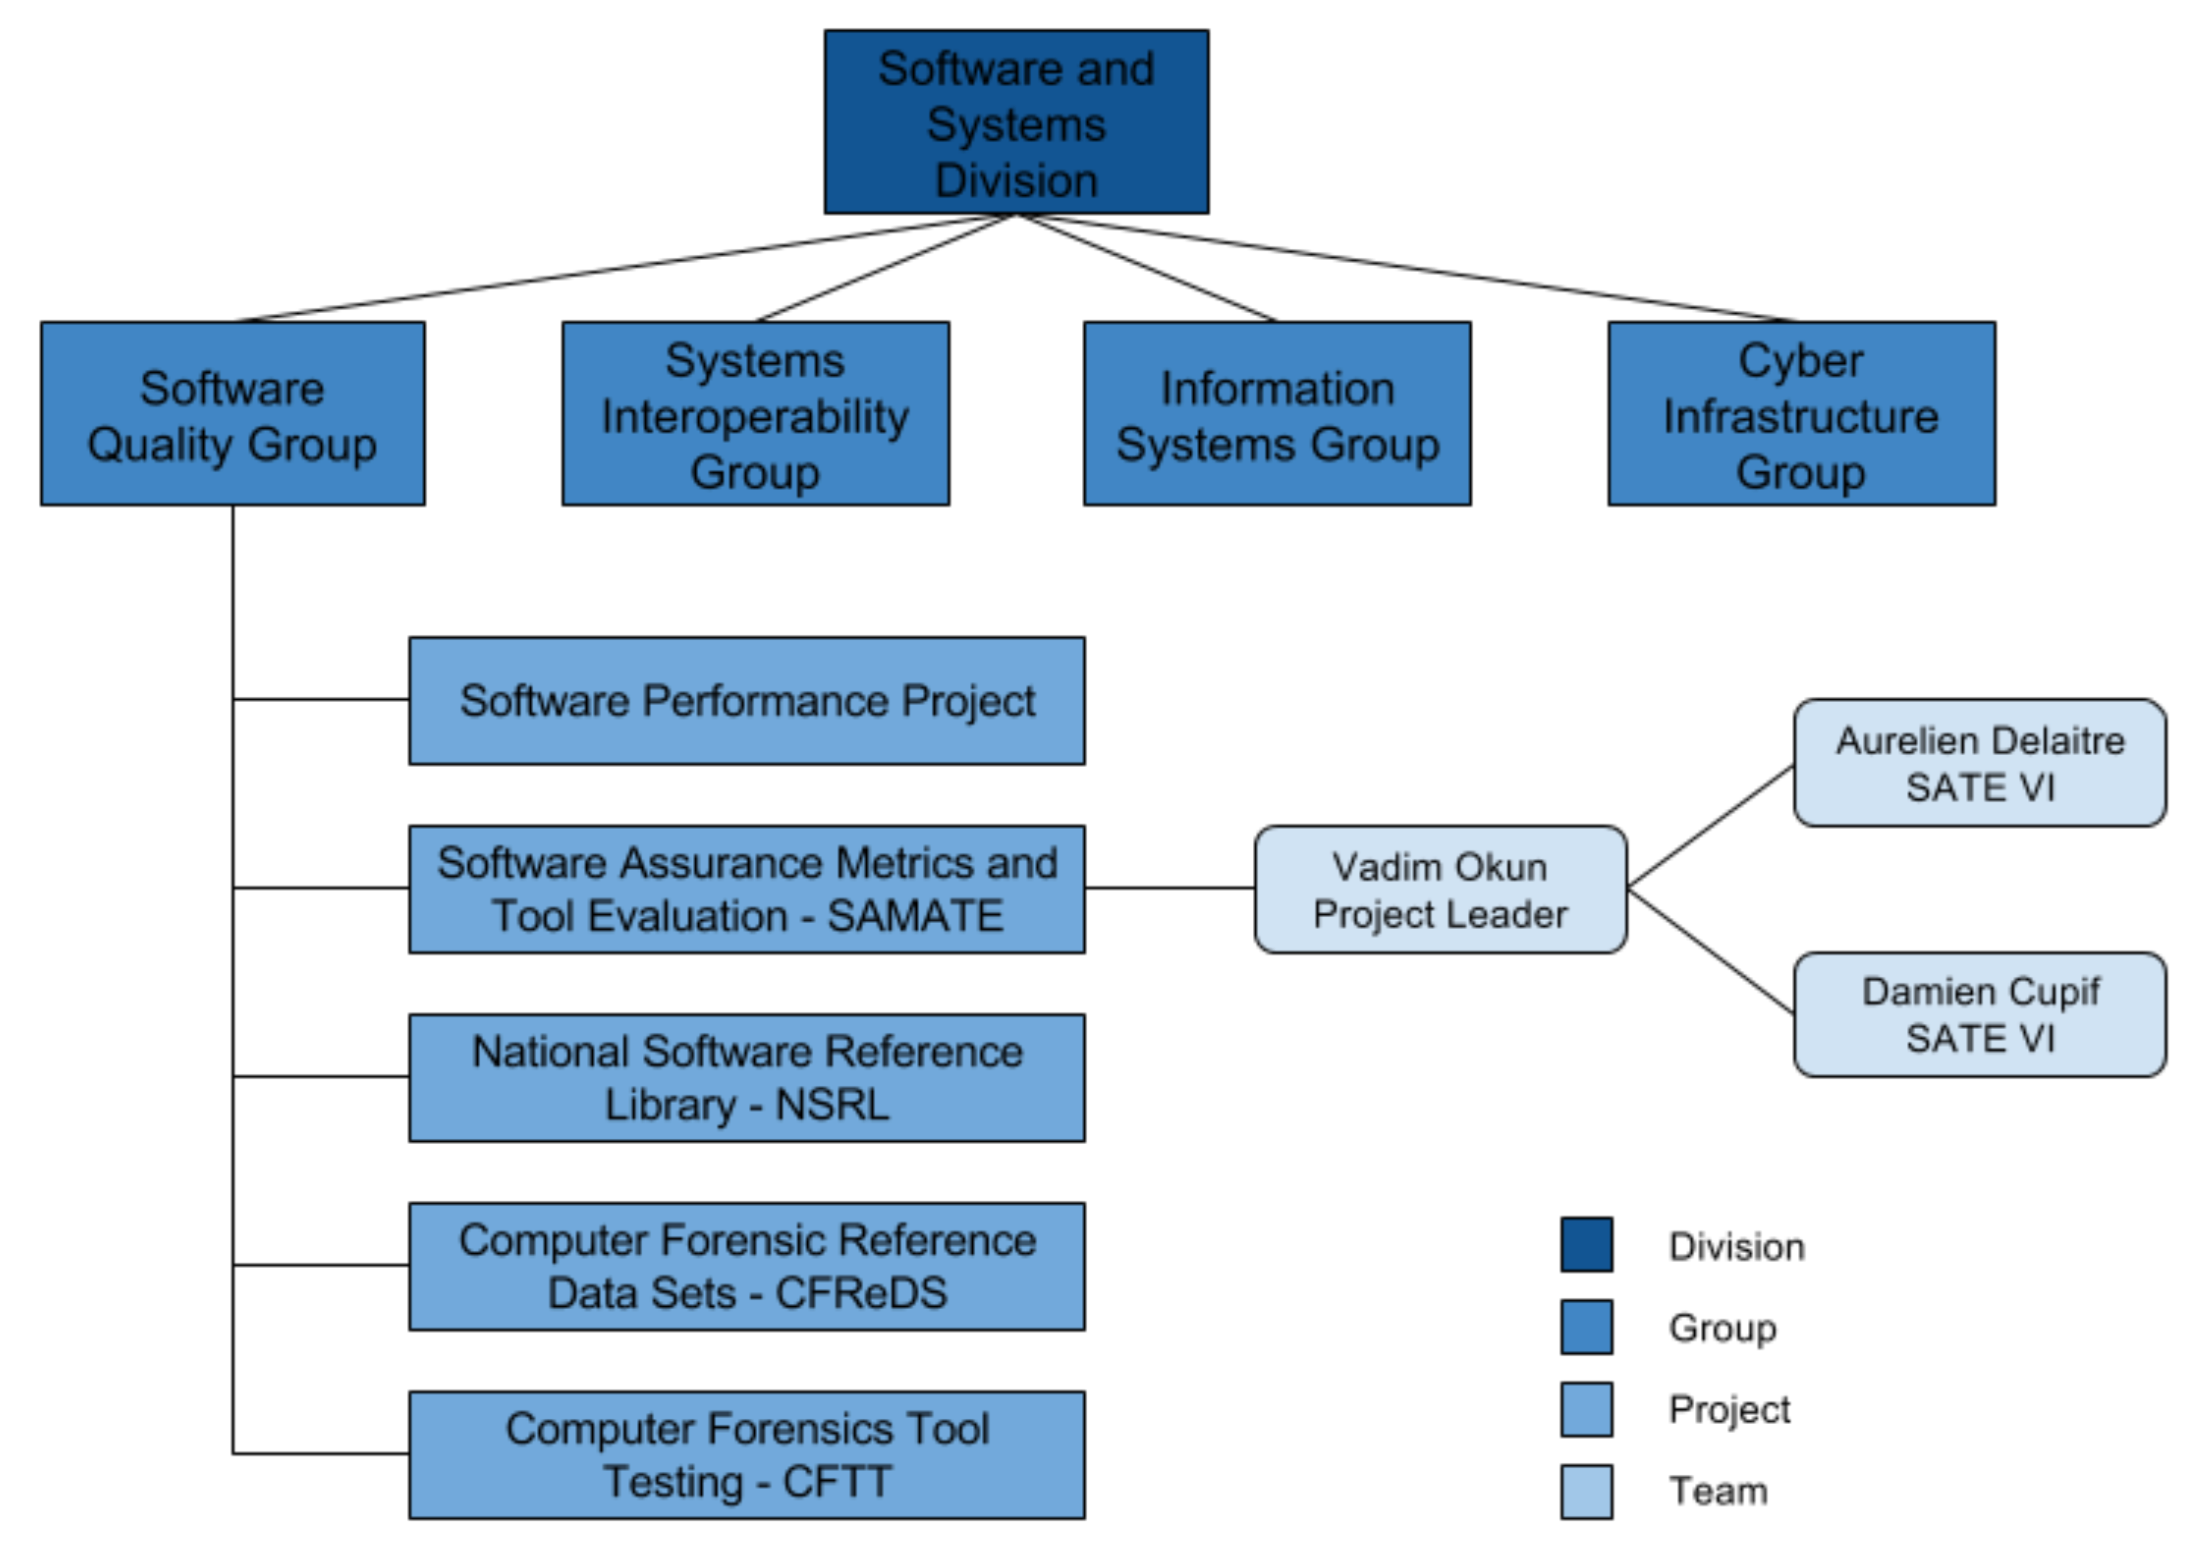
\includegraphics[scale=0.23]{figures/nist-division-organization-chart}
      \caption{Software and Systems Division Organization Chart}
    \end{figure}
  \end{frame}
  
  % Display fully the table of contents once
  \section*{Outline}
  \begin{frame}[noframenumbering, plain]{Outline}
    \tableofcontents[hideallsubsections]
  \end{frame}

  % Beginning of section
  \section{An Introduction to Static Analysis Tool Evaluation}
  
  \subsection{The Need for Software Assurance}
  
  \begin{frame}[standout]
    \begin{quote}
      `` Software is eating the world. ''\\
      --- Marc Andreessen
    \end{quote}
  \end{frame}
  
  \begin{frame}{General Facts About Software}
    \pause
    \begin{description}
      \item[Fact 1:] Software is \textbf{everywhere} and \textbf{powers critical infrastructures} in our everyday lives\\
    \end{description}
    \pause
    \begin{center}
    We trust software blindly, and yet \ldots
    \end{center}
    \vspace{-1.3em}
    \pause
    \begin{description}
      \vfill  
      \item[Fact 2:] Software has \textbf{bugs}
    \end{description}
    \pause
    \vfill
    \begin{definition}
      \vspace{0.3em}
      A \textcolor{mLightGreen}{bug} is a design fault, a defect in a system that may or may not lead to its \textbf{unexpected behavior}.
    \end{definition}
    \vfill
  \end{frame}

  \begin{frame}{Is that a serious issue?}
    \vspace{0.5em}
    \begin{figure}
      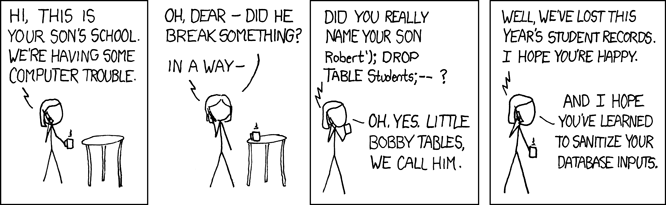
\includegraphics[scale=0.6]{figures/exploits_of_a_mom}
      \caption{Exploits of a Mom}
    \end{figure}
  \end{frame}
  
  \begin{frame}{What can we do?}
    \vspace{-1.4em}
    \begin{columns}[b]
      \begin{column}{0.5\textwidth}
        \begin{figure}
          \centering
          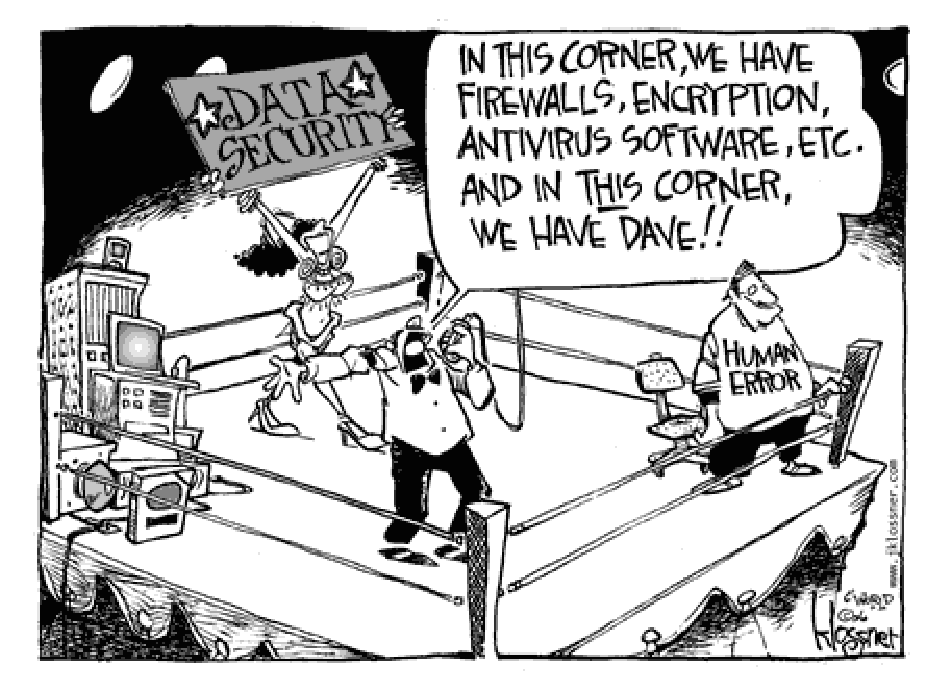
\includegraphics[scale=0.38]{figures/dave}
        \end{figure}
      \end{column}
      \begin{column}{0.5\textwidth}
        But wait \ldots{} we already have:
        \begin{itemize}
        \item firewalls,
        \item antivirus software,
        \item intrusion detection systems,
        \item and more!
        \end{itemize}
        \pause
        Stop, \textbf{treating the symptoms} is not enough!
      \end{column}
    \end{columns}
    \centering
    \vfill
    \pause
    {\LARGE $\to$ We MUST build \alert{better software} in the first place!}
  \end{frame}

  \subsection{What is Static Analysis?}

  \begin{frame}[standout]
    \begin{changemargin}{-2cm}{-2cm}
    \vspace{-0.2cm}
    \begin{figure}
      \centering
      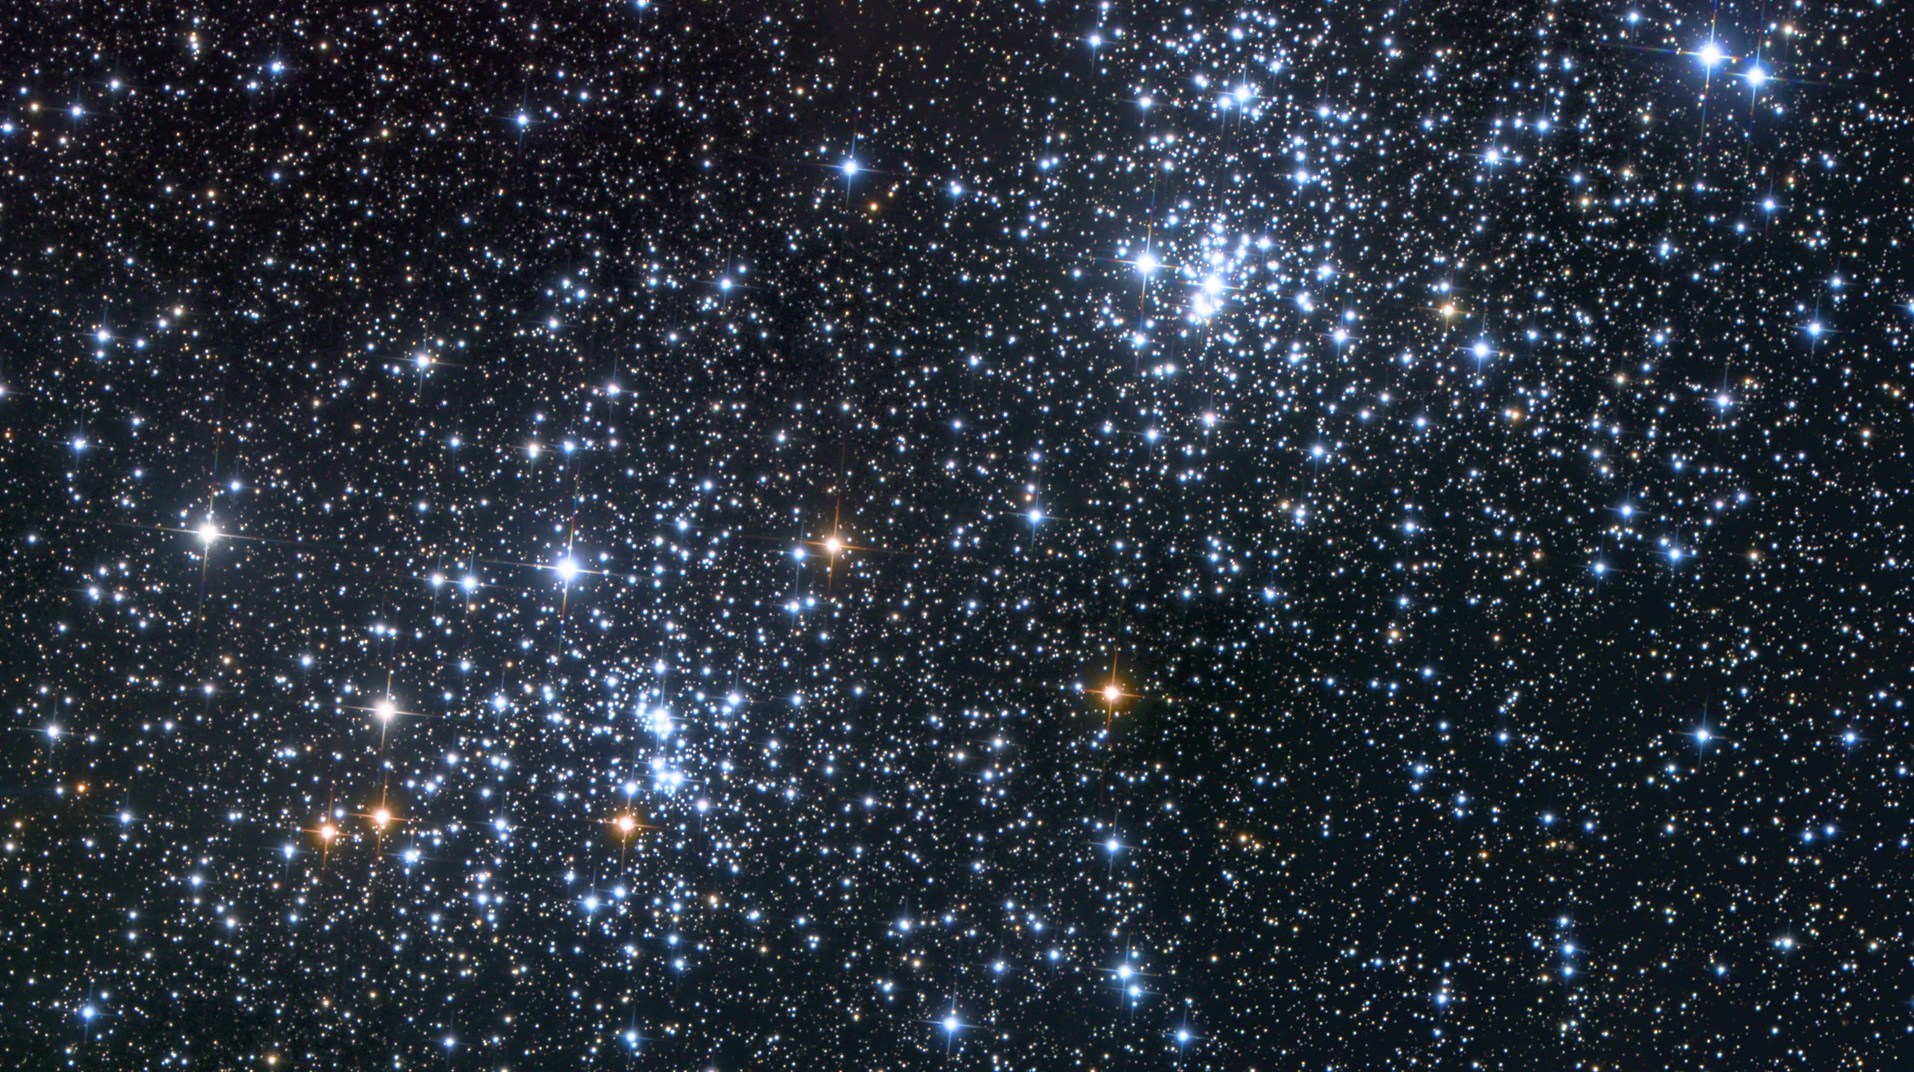
\includegraphics[scale=0.24]{figures/universe}
    \end{figure}
    \end{changemargin}
  \end{frame}

  \begin{frame}{What is Static Analysis?}
    \begin{quote}
      \begin{flushright}
        ``The term \alert{static analysis} refers to any process\\ for assessing code \textbf{without executing it}''\\
        --- Brian Chess, Jacob West
      \end{flushright}
    \end{quote}
    \pause
    \begin{figure}
      \centering
      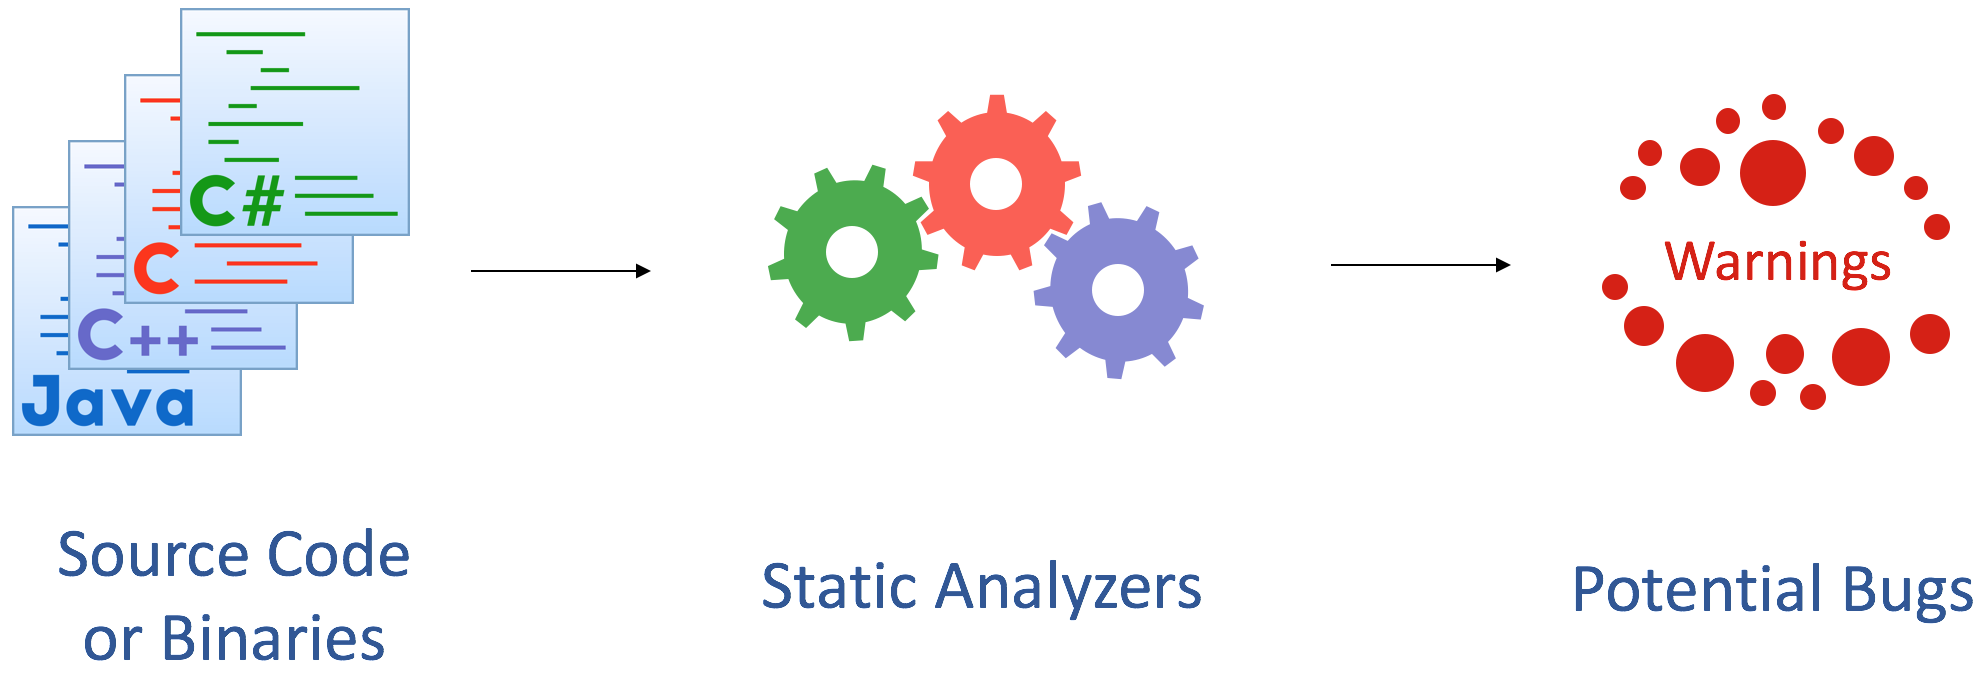
\includegraphics[scale=0.35]{figures/static-analysis}
      \caption{High Level Static Analysis Process Overview}
    \end{figure}
  \end{frame}

  \begin{frame}{Problem solved!}
    \begin{figure}
      \centering
      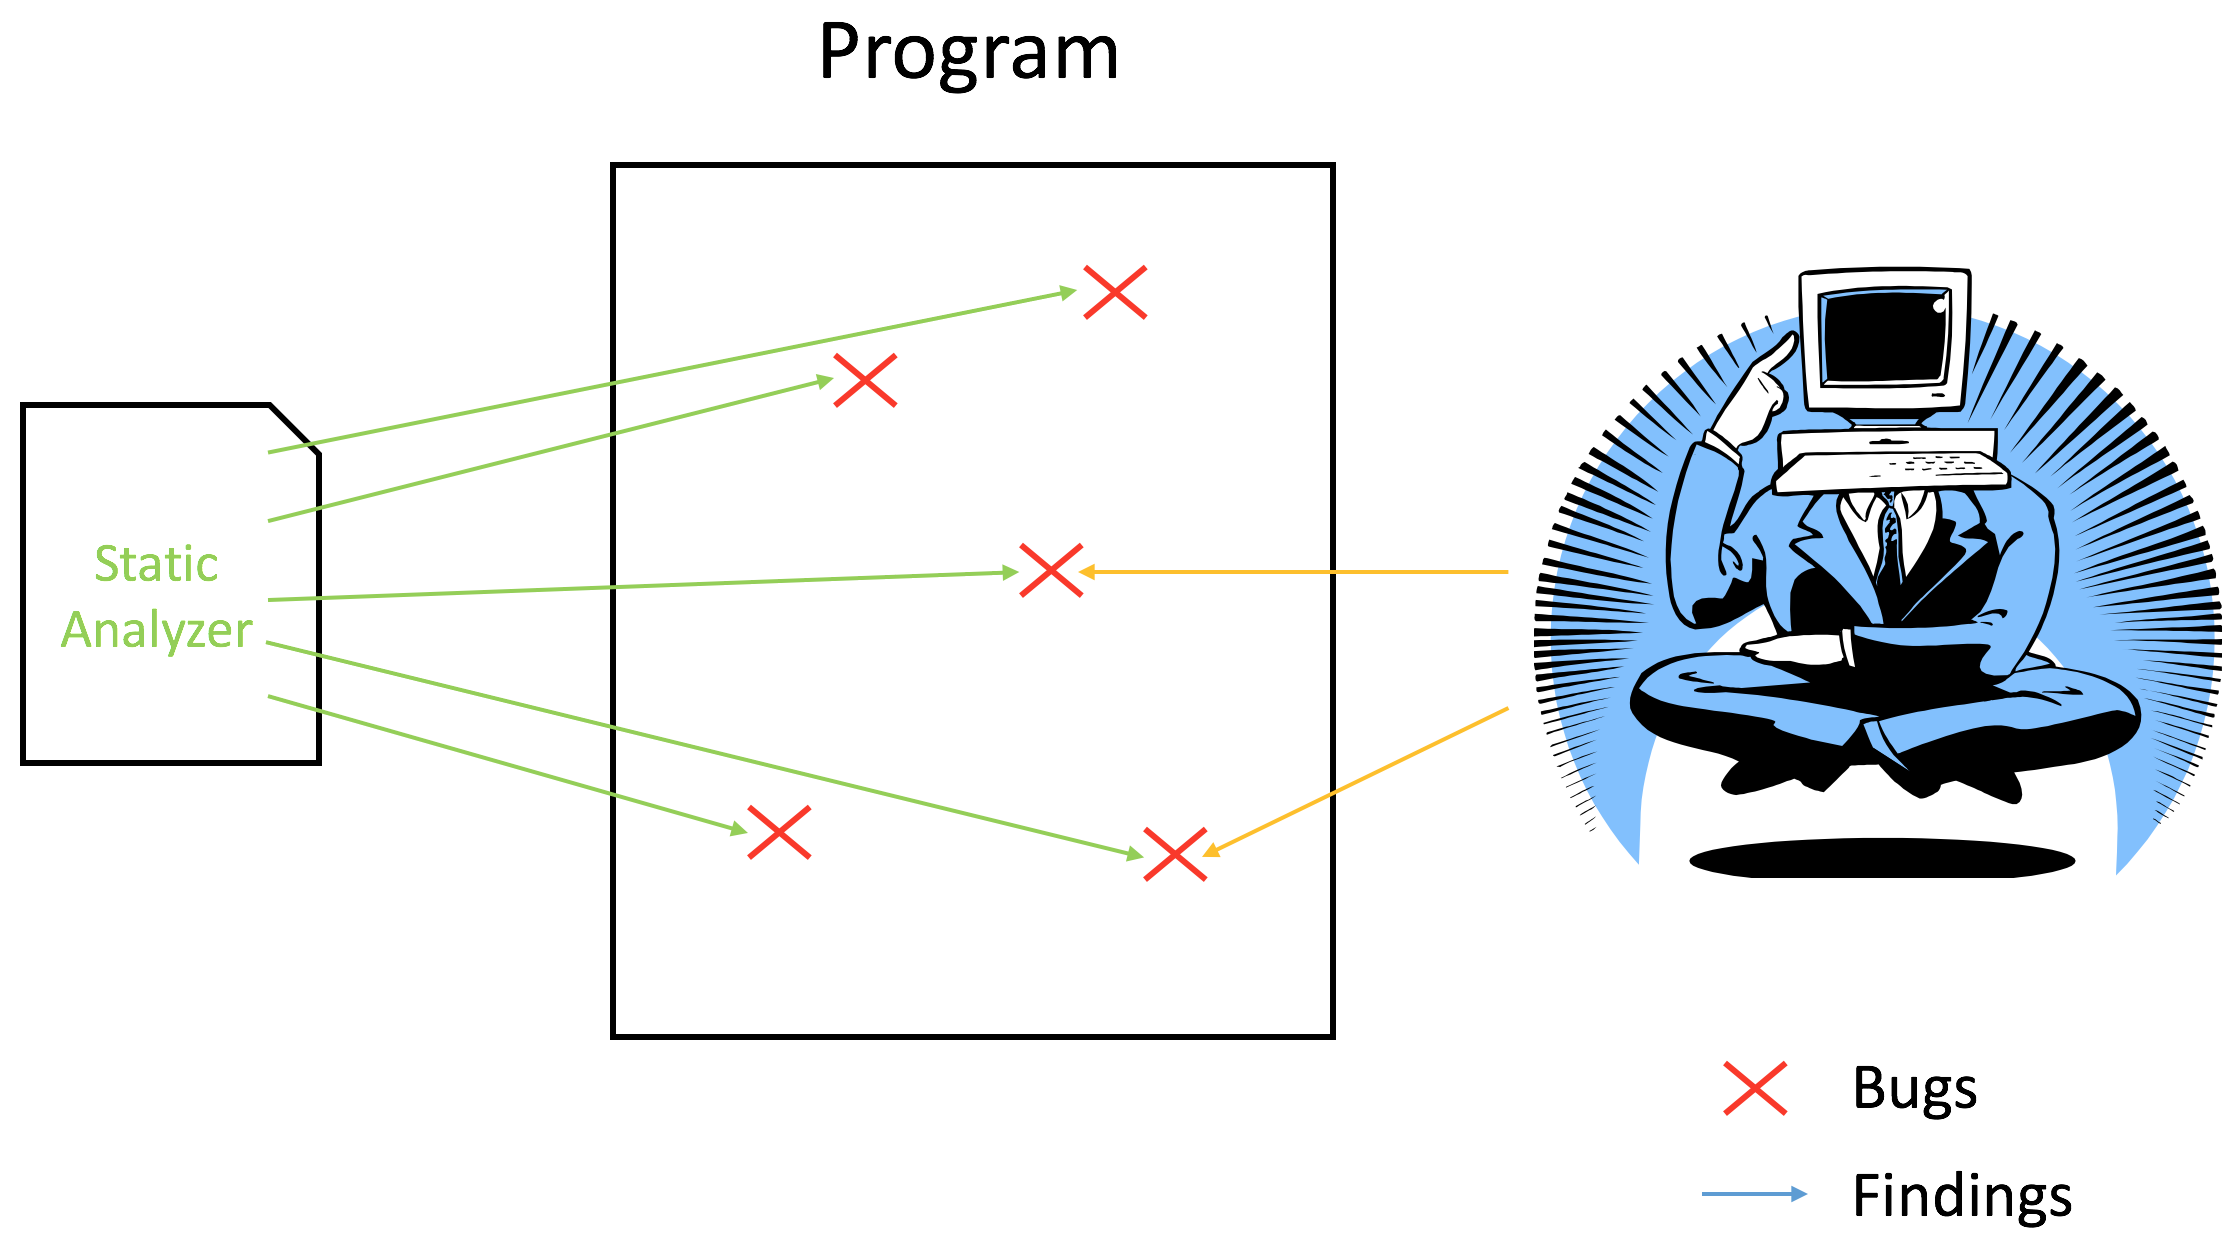
\includegraphics[scale=0.3]{figures/the-dream}
      \caption{The Dream of Every Developer}
    \end{figure}
  \end{frame}

  \begin{frame}{Problem solved! Ugh\ldots{} not quite!}
    \begin{figure}
      \centering
      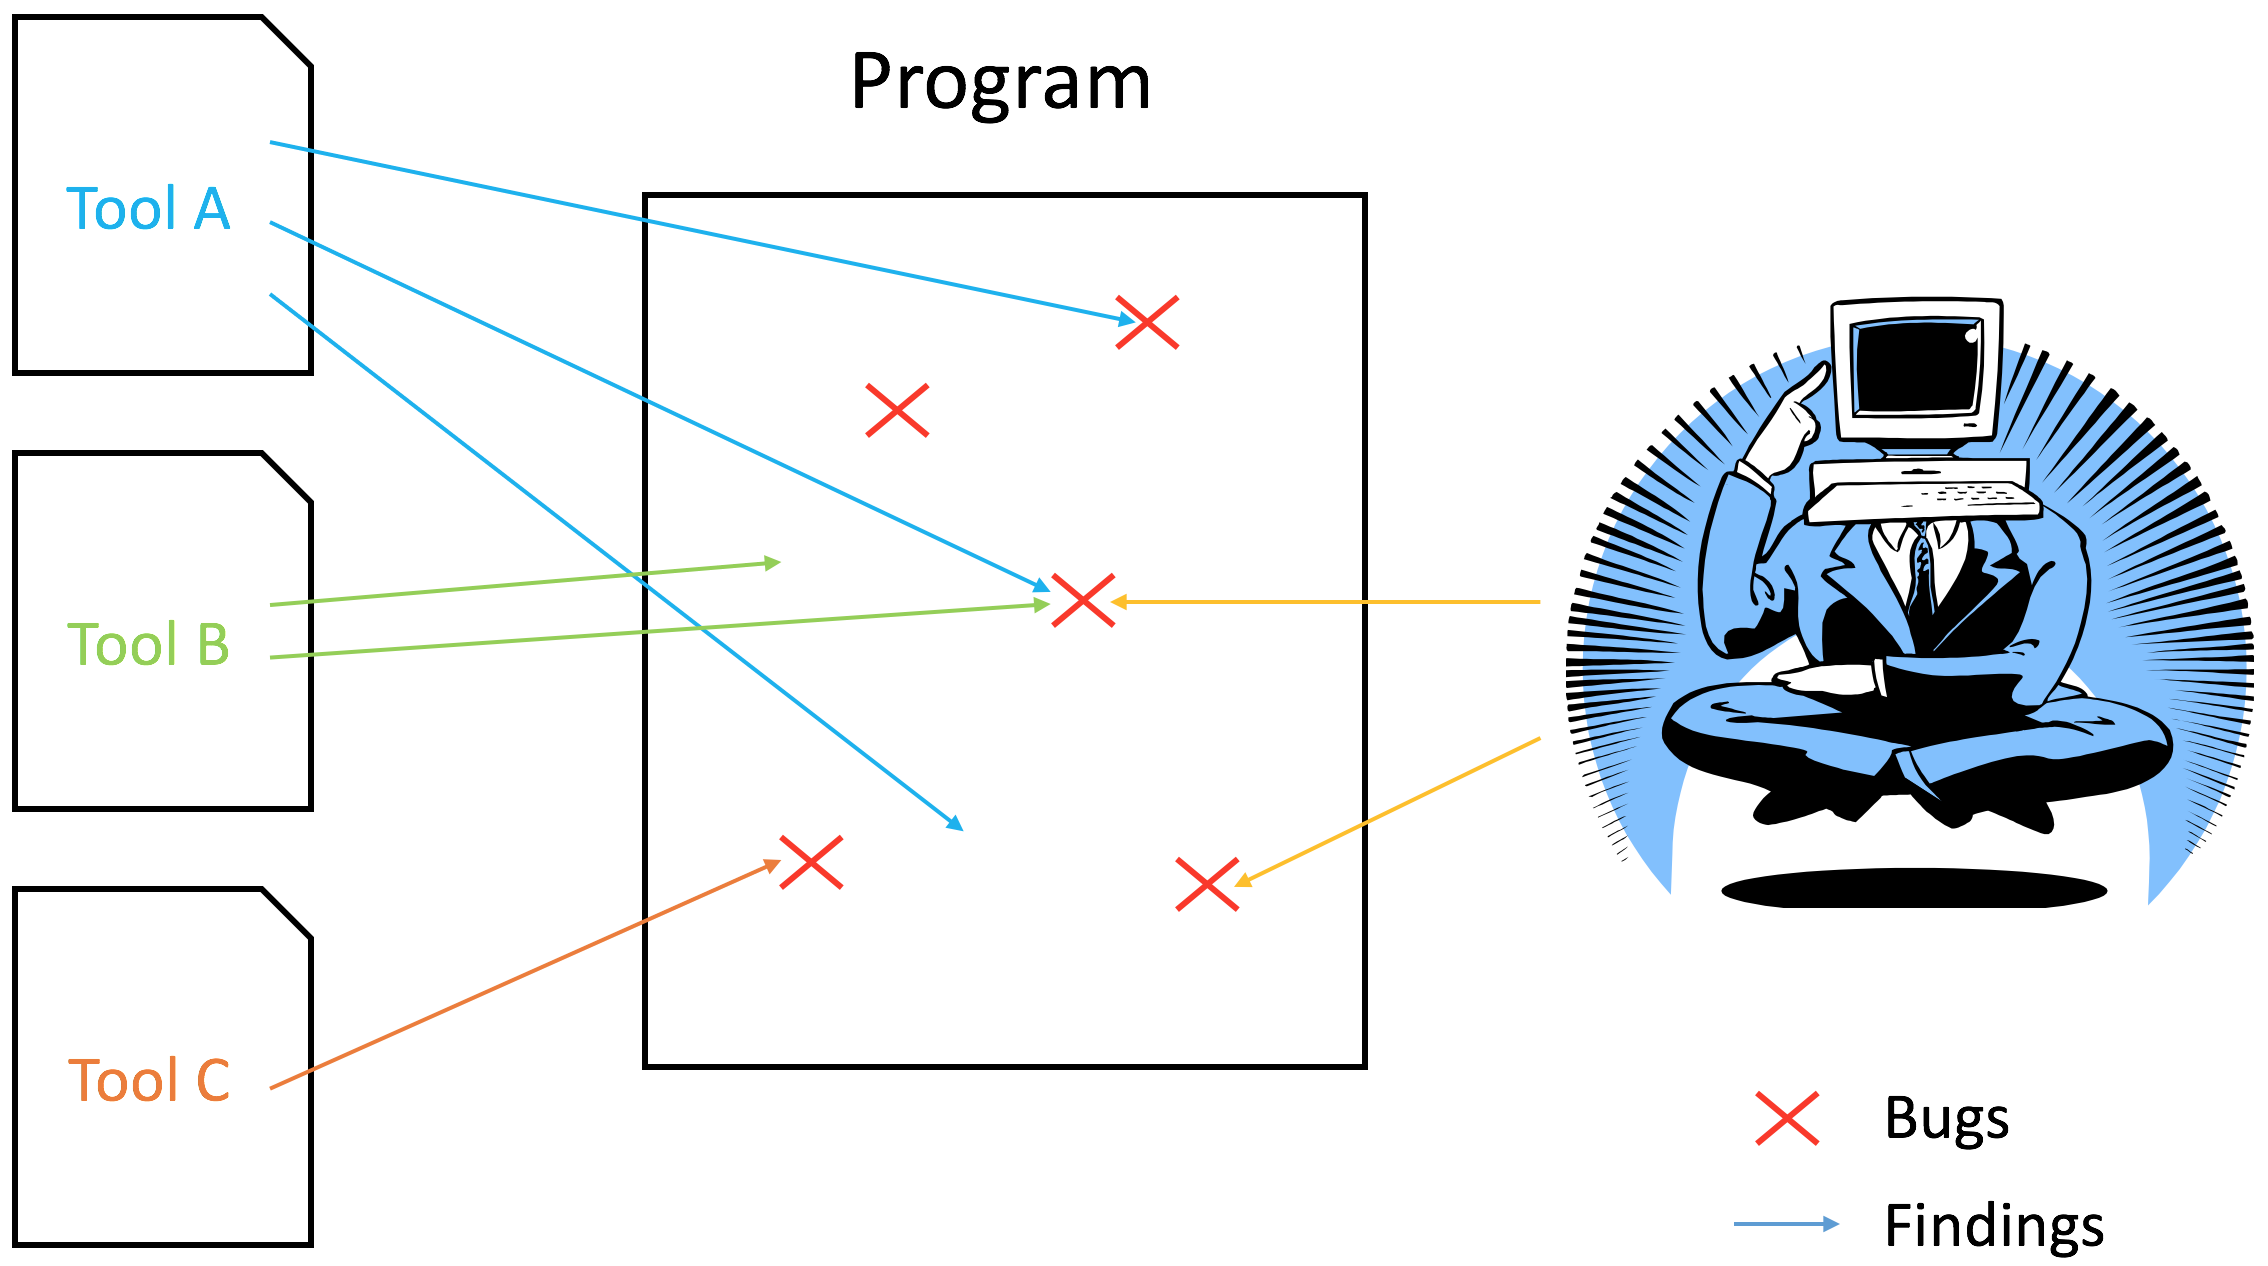
\includegraphics[scale=0.3]{figures/static-analyzers}
      \caption{Static Analyzers Imperfections}
    \end{figure}
  \end{frame}
    
  \subsection{Static Analysis Tool Exposition (SATE) Project}

  \begin{frame}{Static Analysis Tool Exposition (SATE)}
    \textbf{Goal:} \alert{Evaluate the performances of static analyzers}\\
    \pause
    \vfill
    \textbf{Process:}
    \begin{enumerate}
    \item Provide tool makers with \textbf{test suites}
    \item Tool makers run their static analyzers and generate reports
    \item SAMATE team analyze the reports
    \end{enumerate}
    \pause
    \vfill
    \begin{block}{Definitions}
      \vspace{0.3em}
      A \textcolor{mLightGreen}{test suite} is a set of \textbf{test cases}.\\
      \pause
      \vspace{0.3em}
      A \textcolor{mLightGreen}{test case} is a program flawed with vulnerabilities.
    \end{block}
  \end{frame}

  \begin{frame}{Desired Characteristics of Test Suites}
    \begin{figure}
      \centering
      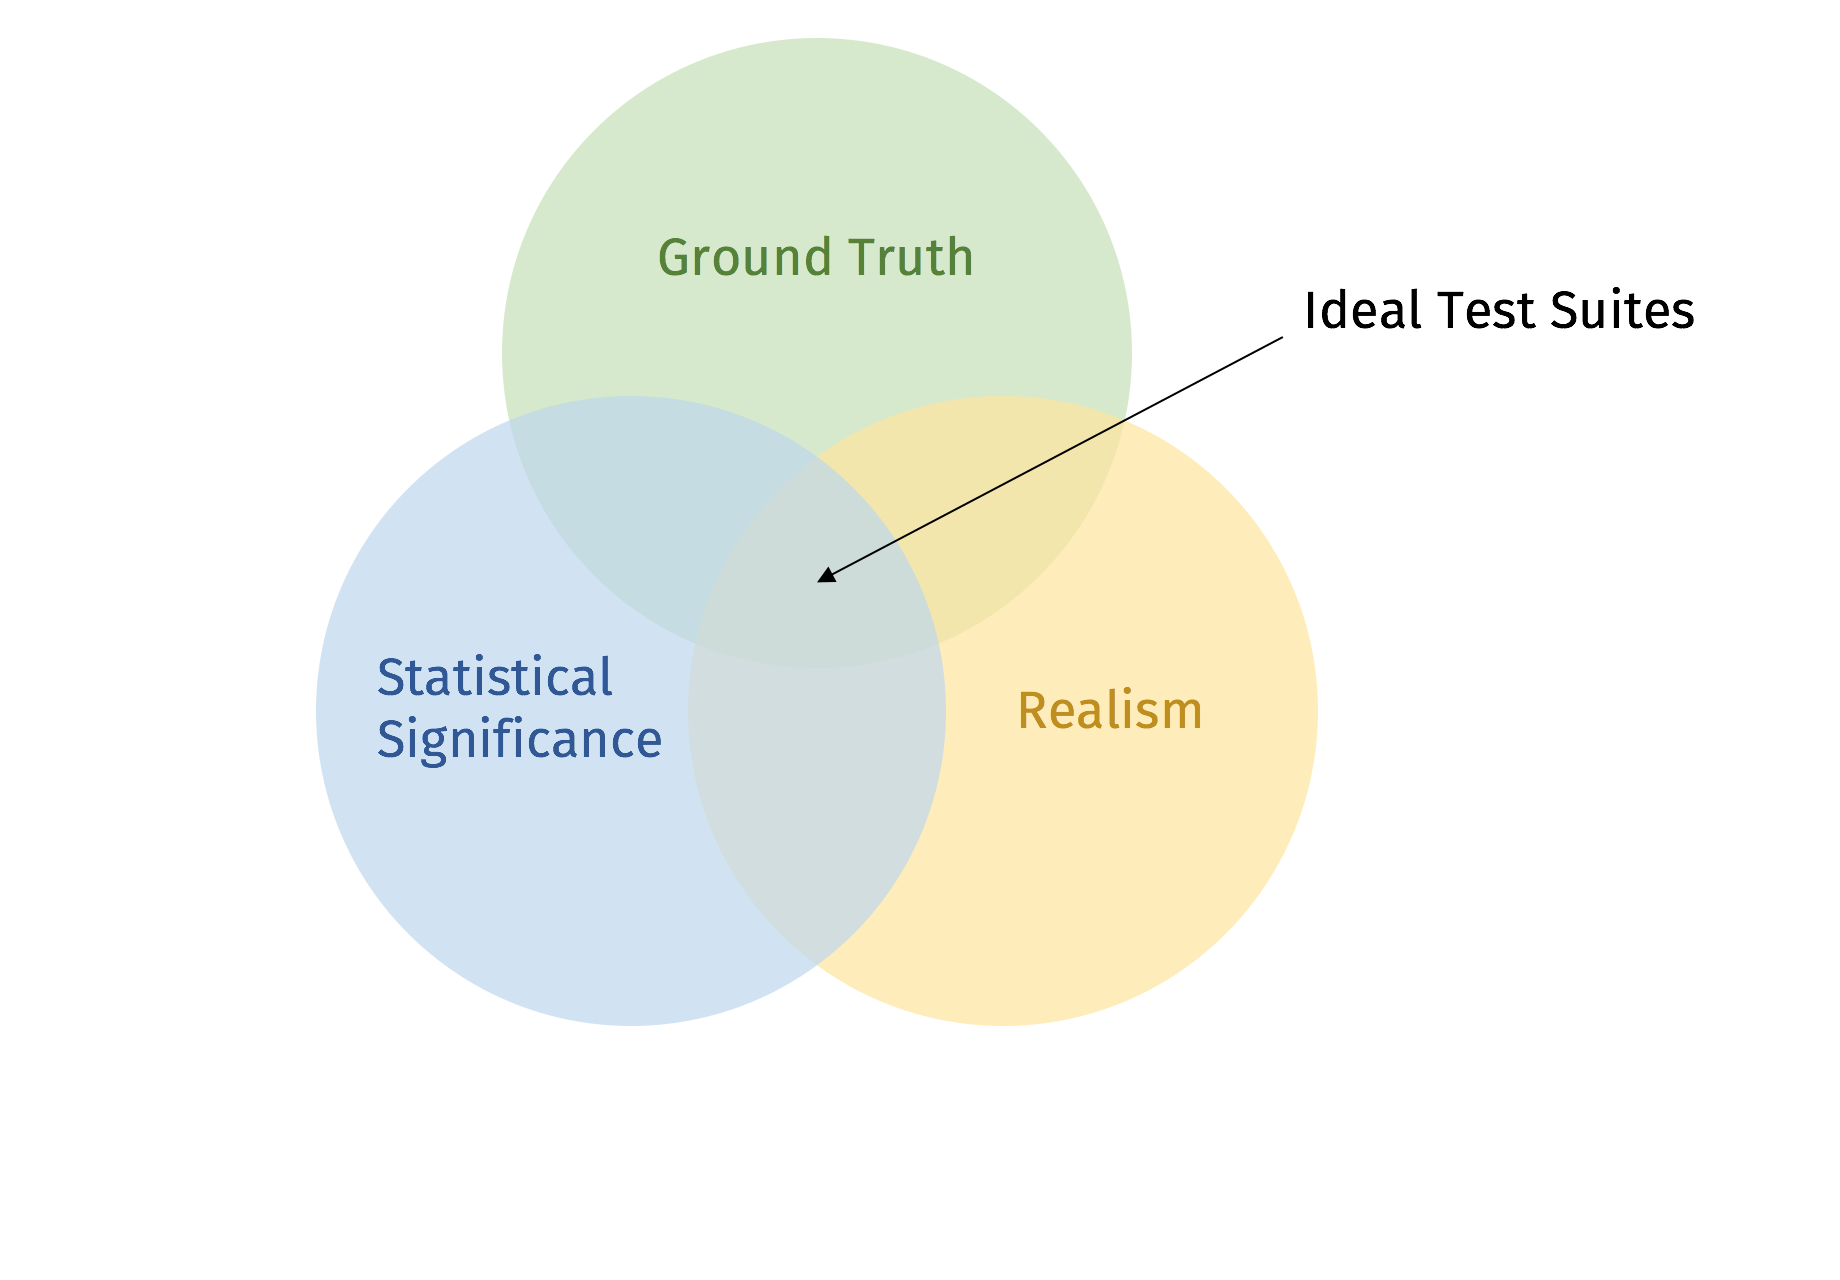
\includegraphics[scale=0.35]{figures/ideal-test-suites}
      \caption{Ideal Test Suites}
    \end{figure}
  \end{frame}

  \begin{frame}{SATE V Test Suites}
    \begin{figure}
      \centering
      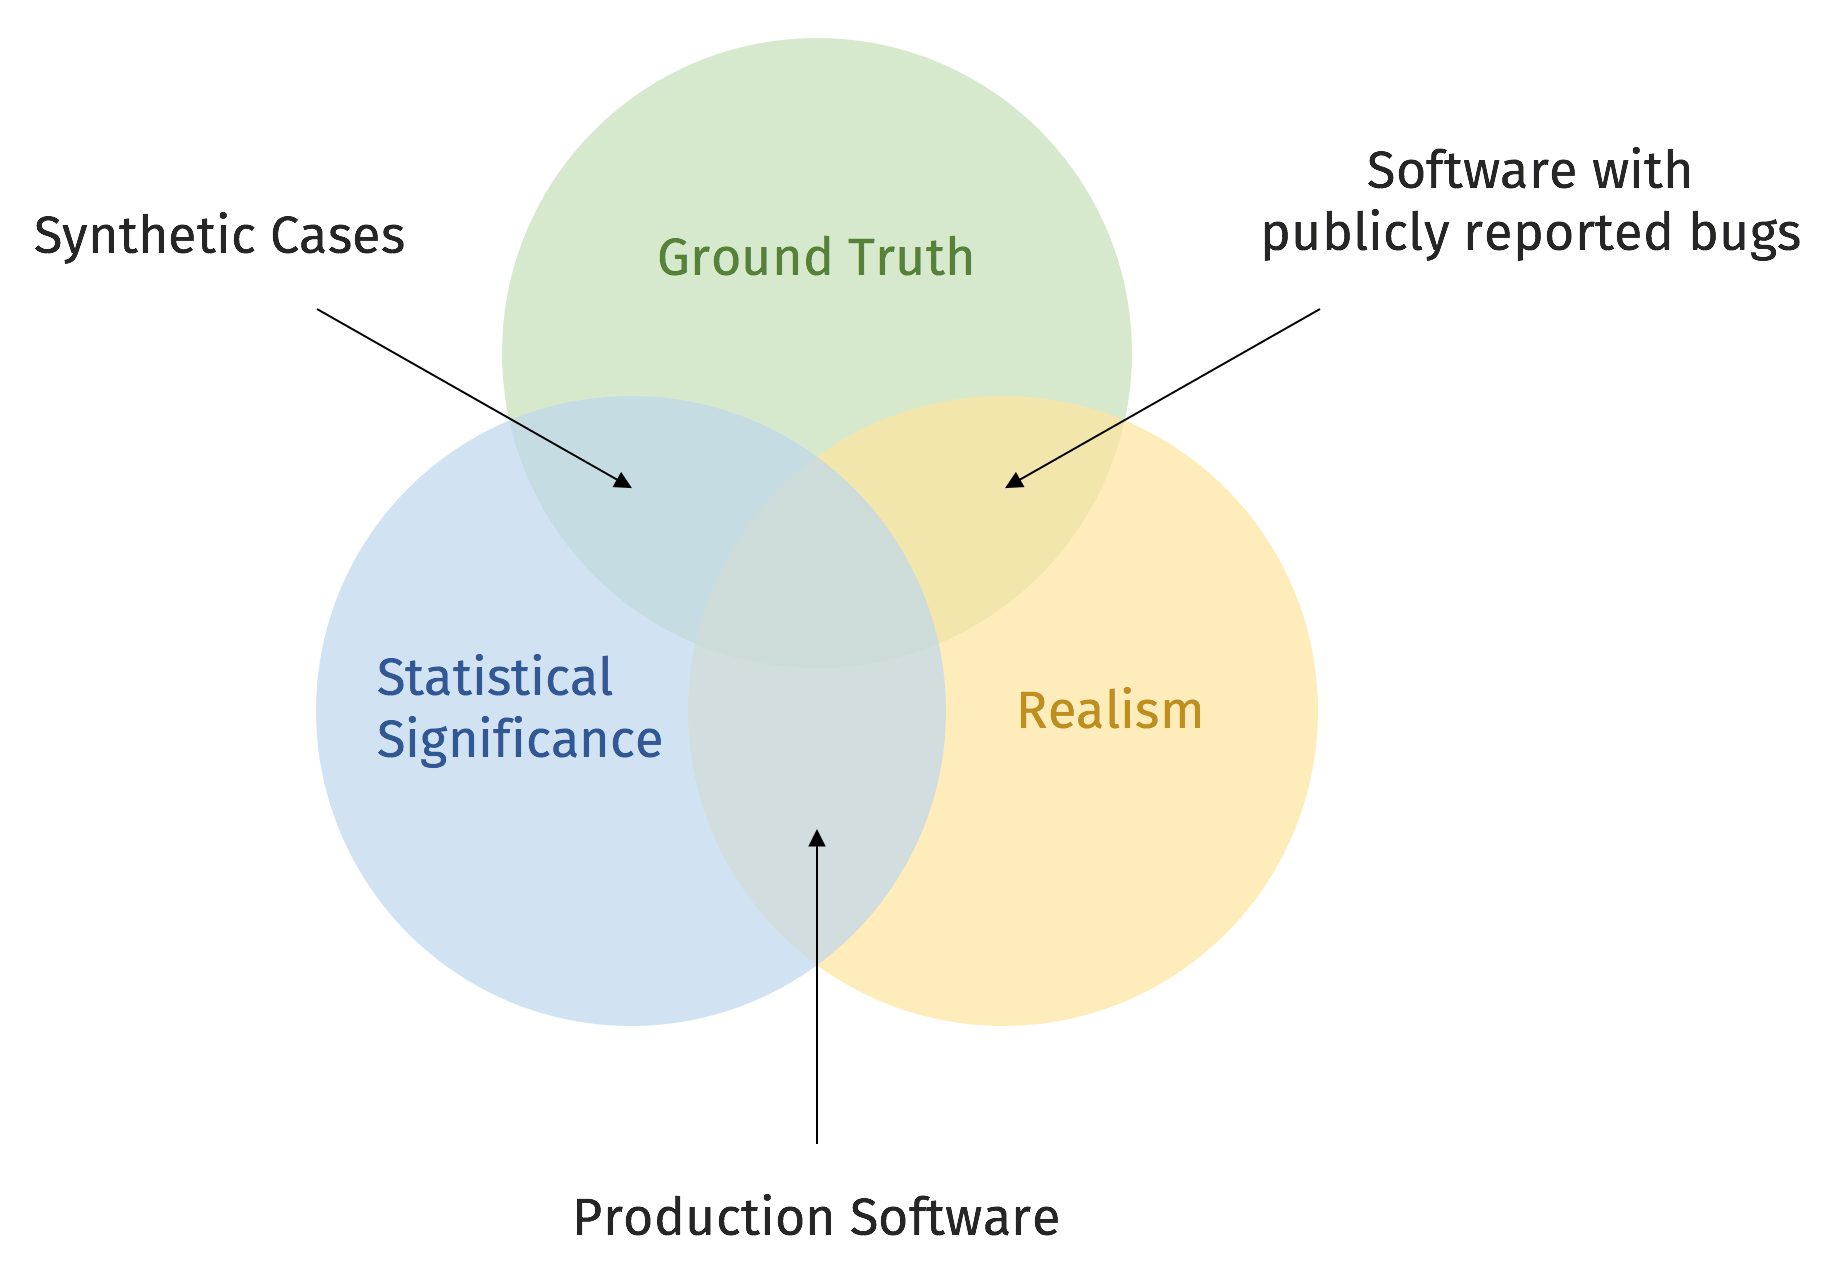
\includegraphics[scale=0.33]{figures/sate-v-test-suites}
      \caption{SATE V Solution}
    \end{figure}
  \end{frame}
  % End of section
  
  % Beginning of section
  \section{SATE VI Test Case Development}

  \subsection{Challenges and Goals}

  \begin{frame}{Project Goals}
    \begin{itemize}
    \setlength\itemsep{1em}
    \item Produce 2 test suites, a \textbf{C/C++ track}, and a \textbf{Java track}
    \pause
    \item The test suites must present the following characteristics:
      \vspace{0.3em}
      \begin{itemize}
      \setlength\itemsep{0.5em}
      \item \textbf{Ground Truth} $\rightarrow$ We know where the bugs are
      \item \textbf{Realism} $\rightarrow$ As close as possible to industrial software
      \item \textbf{Statistical Significance} $\rightarrow$ We want a lot of bugs
      \end{itemize}
    \pause
    \item A \textbf{large spectrum of vulnerability types} should be represented chosen from the CWE/SANS Top 25 and the OWASP Top 10
    \end{itemize}
  \end{frame}

  \begin{frame}{Project Challenges}
    \begin{enumerate}
    \item No such test case exist in the nature
    \item Developing test cases from scratch is not an option to achieve realism
    \end{enumerate}
  \end{frame}
  
  \subsection{Opportunities with Vulnerability Injection Techniques}
  \subsection{Action Plan for Success}
  % End of section

  % Beginning of section
  \section{A Focus on LAVA, a Large-scale and Automated Vulnerability Addition Software}
  \subsection{LAVA Process Overview}
  \subsection{Using LAVA: Pros and Cons}
  \subsection{LAVA Reverse Engineering and Extension}
  % End of section

  % Beginning of section
  \section*{Conclusion}
  % End of section
  
  \begin{frame}{Acknowledgments}
  \end{frame}

  \begin{frame}{References}
  \end{frame}

  \begin{frame}[standout]
    \begin{huge}
      Thank you for your attention!\\\alert{Questions?\\}
    \end{huge}
    \vspace{2.5em}
    \begin{scriptsize}
      For any follow-up, feel free to contact me at\\
      damien.cupif@nist.gov
    \end{scriptsize}
  \end{frame}

  \end{document}
